\documentclass[12pt,a4paper,twoside]{article}

\usepackage[utf8]{inputenc}
\usepackage[T1]{fontenc}
\usepackage{amsmath,amssymb,amsthm}
\usepackage{libertine}
\usepackage{fourier}
\usepackage{graphicx}
\usepackage{framed}

\setlength{\voffset}{-28.4mm}
\setlength{\hoffset}{-1in}
\setlength{\topmargin}{20mm}
\setlength{\oddsidemargin}{25mm}
\setlength{\evensidemargin}{25mm}
\setlength{\textwidth}{160mm}

\setlength{\parindent}{0pt}

\setlength{\textheight}{235mm}
\setlength{\footskip}{20mm}
\setlength{\headsep}{50pt}
\setlength{\headheight}{0pt} 

\newcommand\var[1]{{\operatorname{#1}}}
% \var{eval}
% \var{span}
% \var{Hom}
% \var{Der}
% Composition = .
% \delta_{i,j} Kronecher delta
\newcommand\Z[1]{\nicefrac{\integers}{#1\integers}}

%% General things
%       
        \newcommand\mkset[2]{\left\lbrace#1\,|\, #2\right\rbrace}
        \DeclareMathOperator\diag{\text{diag}}

% Number Sets
%
        \DeclareMathOperator\naturals{\mathbb N_0}
        \DeclareMathOperator\posnats{\mathbb N_{>0}}
        \DeclareMathOperator\integers{\mathbb Z}
        \DeclareMathOperator\rationals{\mathbb Q}
        \DeclareMathOperator\reals{\mathbb R}
        \DeclareMathOperator\complex{\mathbb C}

% Definitional Equality
%
        \DeclareMathOperator\defeq{\overset{\text{def}}=}


% Standard Varieties and related constructions
%
        \DeclareMathOperator\proj{\mathbb P}
        % projective variety for some ideal
        \DeclareMathOperator\V{\mathcal V}
        \DeclareMathOperator\I{\mathcal I}


% Morphism Arrows
%
        \newcommand\hookr\hookrightarrow  
        \newcommand\hookl\hookleftarrow  

%% Polynomial things
%
        \DeclareMathOperator\del\partial



\newtheorem{dummy}{dummy}[section]
\newtheorem{proposition}[dummy]{Proposition}
\newtheorem{corollary}[dummy]{Corollary}
\newtheorem{theorem}[dummy]{Theorem}
\newtheorem{lemma}[dummy]{Lemma}

\theoremstyle{definition}
\newtheorem{definition}[dummy]{Definition}

\theoremstyle{remark}
\newtheorem{example}[dummy]{Example}
\newtheorem{remark}[dummy]{Remark}


\newenvironment{todo}{
  \begin{framed}
  \textbf{TODO}
  \begin{itemize}
}{
  \end{itemize}
  \end{framed}
}


\begin{document}

\pagestyle{empty}
\begin{titlepage}
\begin{center}

\includegraphics{TUMlschwarz.png}\\[3mm]
\sf
{\Large
  Technische Universit\"at M\"unchen\\[5mm]
  Department of Mathematics\\[8mm]
}
\normalsize
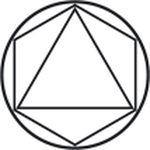
\includegraphics{TUMlMschwarz.png}\\[15mm]

Bachelor's Thesis\\[15mm]

{\Huge
  The 27 Lines on a Cubic Surface
}
\bigskip

\normalsize

Long Huynh Huu <long.huynh-huu@tum.de>
\end{center}
\vspace*{75mm}

Supervisor: Christian Liedtke <liedtke@ma.tum.de>
\medskip

Advisor: Christian Liedtke <liedtke@ma.tum.de>
\medskip

Submission Date: October 27th, 2014

\end{titlepage}

%%%% The following has to be signed by hand!

\vspace*{150mm}

I assure the single handed composition of this bachelor's thesis only supported by declared resources.
\bigskip

Garching, 
\newpage


\section*{Zusammenfassung}
%TODO: Auf Deutsch
xxxxxxxxxxxx deutsche Zusammenfassung xxxxxxxxxx

In this Bachelor thesis I will prove in full detail the existence of 27 lines on an arbitrary smooth cubic in projective $n$-space over an algebraically closed field $k$.

\newpage
\tableofcontents
\newpage

\pagenumbering{arabic}
\pagestyle{headings}


% \section{Change of coordinates}

\subsection{Notes to myself}

In this section I introduce definitions and hands-on examples to work with geometric objects in the language of scheme theory, or maybe I'll just drop the generalities and work with elementary algebra.
Particular goals are
\begin{itemize}
\item the definition of what a change of coordinates means precisely and work out the details to use it without regret in the proof of the main result.
\item the definition of what it means for a variety to contain a doubled line. In scheme theoretic language it is as simple as saying, that this variety has a subscheme isomorphic to a doubled line! Again, I might drop the notion of schemes, or work with it.
\end{itemize}
So this text also aims to be educational and close the gap between the intuitive and the technical.

It might be interesting to
\begin{itemize}
\item introduce the category of varieties and rational functions. \textbf{If needed}.
\end{itemize}

\subsection{Affine linear transformations of affine space}

An important notion which will appear again and again is the change of coordinates.
In affine space one thinks of a linear transformation $T:\affine^n_k \to \affine^n_k$.
Now observe the effect of such a transformation on a hypersurface $V(I)$, $I = (f)$:
$ T(V(I)) = \{ Tx \in k^n: f(x) = 0 \} = \{y \in k^n : f(T^{-1}y) = 0\}$
So one may define a linear transformation on a variety by precomposing the inverse to the polynomial functions.
But let me suggest a different definition of linear transformation which does not necessarily require $T$ to be invertible and which is compatible with the scheme theoretic notion of a morphism.

\begin{definition} Let $A = (a_{ij}) \in M(n,k)$ be a $n\times n$-matrix. Then we can define a homomorphism of polynomial rings
\begin{align}
T^\#_A : k[X_1,.. X_n] &\to k[X_1,.. X_n], \\
X_i &\to \sum_{j=1}^n a_{ij}X_j.
\end{align}
\end{definition}

This induces a morphism $T_A : \affine^n_k \to \affine^n_k$ of affine schemes. Indeed, this definition does what we expect.

\begin{proposition} By Hilbert's Nullstellensatz a point $(x_1,..x_n) \in k^n$ corresponds to a maximal ideal $(X_1-x_1,.. X_n-x_n) \subset k[X_1,..X_n]$.
$T_A$ maps the subscheme $V(X_1-x_1,..X_n-x_n)$ to $V(X_1-y_1,..X_n-y_n)$ where $(y_1,..y_n) = A(x_1,..x_n)$.
\end{proposition}

\begin{proof} If $A$ is invertible, we basically apply the Gauß-Jordan algorithm....
\end{proof}

Don't forget the translations: $X_i \mapsto X_i + t_i$.
Together we get affine linear transformations.


\subsection{Rational maps}

Fancy category language here...

\section{General facts}

\subsection{projective space}

In order to do geometry we need to explain what points, lines, surfaces are, and this can be done in several ways, synthetically or analytically.

There are several formulations of projective space, with varying degree of generality, and for our purposes I have chosen the one in terms of homogeneous coordinates.

Let $k$ be an algebraically closed field and $n$ a natural number.
The projective space $\proj^n_k$ is a topological space given as set by  $k^{n+1} - \{ 0 \}$ modulo the relation $X=(x_0,..x_n) \sim Y=(y_0,..y_n)$ if and only if $X$ and $Y$ are linearly dependent (as vectors in $k^{n+1}$). The equivalence class of $X$ will be denoted $[x_0:x_1:..:x_n]$.

The topology is given by the closed subsets
\begin{equation}
\V(I) =
\mkset{ [x_0:..x_n] \in \proj^n_k}
      { \forall f\in I \text{ homogeneous}, f(x_0,..x_n) = 0}
\end{equation}
for homogeneous ideals $I$ of the polynomial ring $k[x_0,..x_n]$.
The topology is known as Zariski's topology.
Because $k[x_0,..x_n]$ is a Noetherian ring, every ideal is finitely generated and in particular every homogeneous ideal is finitely generated by homogeneous elements.
So we may say that a closed set consists precisely of the points in projective space where a finite set of homogeneous ideals vanish.

In this framework I want to identify geometric objects with homogeneous ideals of $k[x_0,..x_n]$.
However, most of the time it is easier to speak of the closed subsets of projective space, instead of the ideal $I$, and $I$ itself can be recovered by means of Hilberts's Nullstellensatz in the form of its radical.

A \emph{hypersurface} is given by one equation $f=0$ for $f\in k[x_0,..x_n]$, and its set of points is $\V(f)$.
In case of $f$ being a linear form we call $\V(f)$ a \emph{hyperplane}.

A line is determined by $n-1$ $k$-linearly independent linear forms and a point by $n$ $k$-linearly independent linear forms.

\subsection{partial derivatives}

In this section we discuss partial derivatives -- a useful algebraic tool to obtain some geometric properties.
 % TODO

\begin{definition}[partial derivative]
Let $D : k[x_0,..x_n] \to k[x_0,..x_n]$ be a derivation over $k$, i.e. a homomorphism of $k$-modules which satisfies the Leibniz rule $D(xy) = xDy+yDx$ for $x,y \in k[x_0,..x_n]$. Furthermore let $D(h) \in k$ for every linear form $h$. We call such a derivation a \emph{partial derivative}.
\end{definition}

\begin{example}
The standard example for partial derivatives are of course the partial derivates with respect to one of the variables $x_i$, defined as $\del_{x_i}(x_j) = \delta_{i,j} := \begin{cases} 1, & \text{ for } i = j \\ 0, & \text {otherwise.} \end{cases}$
\end{example}

\begin{example}
For any monomial $\{ h_i\}_{i=0}^n$ basis of $\bigoplus_{i=0}^n kx_i \subset k[x_0,..x_n]$ we obtain a family of partial derivatives $\{ \del_{h_i} \}_{i=0}^n$ for which $\del_{h_i}(h_j) = \delta_{i,j}$ holds. The construction goes as follows: Let $M = (a_{i,j})  \in k^{(n+1)\times(n+1)}$ be the base change matrix and $M^{-1} = (\widetilde a_{i,j})$ be its inverse.
This just means $h_i = \sum_{j=0}^n a_{i,j} x_j$ and hence $\del_{x_k}(h_i) = a_{i,k}$.
From $\delta_{i,j} = \sum_{k=0}^n a_{i,k}\widetilde a_{k,j}
= \sum_{k=0}^n \del_{x_k}(h_i) \widetilde a_{k,j}$ it is obvious that we need to define

\begin{equation}
\del_{h_j} = \sum_{k=0}^n \widetilde a_{k,j} \del_{x_k}
\end{equation}

Another write to write this would be
\begin{equation}
\begin{pmatrix} \del_{h_0} \\ \vdots \\ \del_{h_n} \end{pmatrix}
= M^{-T}
\begin{pmatrix} \del_{x_0} \\ \vdots \\ \del_{x_n} \end{pmatrix}
\end{equation}
\end{example}

A useful fact, that allows us to recover a homogeneous polynomial by its partial derivatives is

\begin{proposition}[Euler's formula]
For any $f \in k[x_0,..x_n]$ homogeneous of degree $d$ we have the equality
\[ df = \sum_{i=0}^n \del_{x_i}(f)x_i \]
\end{proposition}
\begin{proof}
By linearity we only need to prove the monomial case $f = \prod_{i=0}^n x_i^{a_i}$, $a_i$ being integers such that $\sum_{i=0}^n a_i = d$.
\begin{equation}
\sum_{i=0}^n \del_{x_i}(f)x_i
= \sum_{i=0}^n \begin{Bmatrix} \left(\prod_{j\neq i} x_j^{a_j}\right) a_i x_i^{a_i-1} x_i, & \text{ for } a_i > 0
\\ 0, &\text{ for } a_i = 0 \end{Bmatrix}
= \sum_{i=0}^n a_i f = df
\end{equation}
\end{proof}

\begin{corollary}
$\V(\del_{x_0}(f),..\del_{x_n}(f), df) = \V(\del_{x_0}(f),..\del_{x_n}(f))$
\end{corollary}


\begin{lemma}
Let $\del_1,\del_2$ be partial derivatives, then $\del_1.\del_2 = \del_2.\del_1$.
\end{lemma}
\begin{proof}
We only need to prove this for monomials, and we'll perform an induction on the degree.
If $f$ is a monomial of degree less than 2, then $\del_1(\del_2(f)) = 0 = \del_2(\del_1(f))$. 
Now suppose $f = x_if'$ and $\del_1(\del_2(f')) = \del_2(\del_1(f'))$.

\begin{equation}
\del_1.\del_2(x_if') = \del_1(x\del_2(f') + f'\del_2(x)) = 
\del_1(x)\del_2(f') + \del_1(f')\del_2(x) + x\del_1(\del_2(f')) + \underset{=0}{\underbrace{f'\del_1(\del_2(x))}}
\end{equation}
The last term is symmetric in $\del_1,\del_2$ (by assumption).
\end{proof}

\begin{corollary}[Taylor's formula]
Let $f \in k[x_0,..x_n]$ be a polynomial and $f = \sum_{i=0}^d f_i$ its decomposition into homogeneous parts.
Then $f_i = \frac{1}{i!} \sum_{|\bf{\alpha}|=i} \del^{\bf{\alpha}}(f)(0)x^{\bf{\alpha}}$ in multi-index notation.
\end{corollary}
\begin{proof}
% TODO ...
\end{proof}





\subsection{singularities and the tangent plane}

% TODO


\subsubsection{Invariance of singularities under a change of the system of partial derivatives}

Oftentimes it is more convenient to perform base changes to simplify equations and sometimes one can do without, bnut in exchange one needs to introduce more flexible tools.

Remember, in order to study singularities we introduced partial derivatives $\del_{x_i} : k[x_0,..x_n] \to k[x_0,..x_n]$ which satisfied $\del_{x_i}(x_j) = \delta_{i,j}$.

%TODO


\subsection{plane conics -- the question of degeneracy}

A plane conic is a algebraic variety $\V(g)$ given by a quadratic form $g \in k[x_0,x_1,x_2]$. One might ask the question whether the conic is a union of two lines (in which case the conic is called \emph{degenerate}), or in algebraic terms, whether $g$ factors into two linear forms or whether it is irreducible.
Let's turn our attention the an easier question: When is a conic singular?

Assume that the characteristic of our base field $k$ is not 2, then the conic can be written, for appropriate coefficients $a,b,c,d,e,f \in k$ as:
\begin{equation}
g = ax_0^2 + bx_0x_1 + cx_1^2 + dx_0x_2 + ex_1x_2 + fx_2^2
\end{equation}
The singular points are given by the system of equations
\begin{equation}
\del_{x_0} g = \del_{x_1} g = \del_{x_2} g = 0
\end{equation}
which written out in matrix notation, amounts to
\begin{align}
\underset{=:M}{\underbrace{
\begin{pmatrix}
2a & b & e \\
b & 2c & d \\
e & d & 2f
\end{pmatrix}
}}
\begin{pmatrix}
x_0 \\ x_1 \\ x_2
\end{pmatrix}
=
0
\end{align}
We call the matrix $M$.
A singular point $[s_0:s_1:s_2] \in \proj^2_k$ would of course be a non-zero solution of above equation and as such can only exist precisely if the determinant of $M$ vanishes.
So far we have obtained

\begin{corollary}
Let $k$ be a field of characteristic not 2 and $g =  ax_0^2 + bx_0x_1 + cx_1^2 + dx_0x_2 + ex_1x_2 + fx_2^2
\in k[x_0,x_1,x_2]$ be a quadratic form. The conic $\V(g) \subset \proj^2_k$ is singular if and only if
\begin{equation}
\frac 12
\det
\begin{pmatrix}
2a & b & e \\
b & 2c & d \\
e & d & 2f
\end{pmatrix}
= 4acf + bde - ce^2 - ad^2 - b^2f = 0
\end{equation}
\end{corollary}

Incidentally this statement holds true for characteristic 2 as well, even though we need to approach the proof a little differently.
At this point I remind the reader that addition and subtraction are the same in characteristic 2, in the sense that negation operation is just the identity, which will simplify the calculations a little.
The corollary then translates to $g$ having a singular point if and only if $bde + ce^2 +ad^2 + b^2f = 0$.
The set of singular points is by definition the intersection of $V = \V(\del_{x_0}g,\del_{x_1}g,\del_{x_2}g)$ and $\V(g)$, so let's calculate the points in the first variety: Assuming that not all coefficients $b,f,e$ vanish, the only point on $V$ is $[e:d:b]$, as can be seen by Gaussian elimination where we distinguish the cases of $0,1$ or $2$ of the coefficients $b,d,e$ vanishing.
This point $[e:d:b]$ lies on $\V(g)$ iff $0 = g(e,d,b) = ae^2 + bde + cd^2 + dbe + ebd + fb^2 = bde + ae^2 + cd^2 + fb^2$ as desired.
If all of $b,d,e$ vanish, then $V$ is the whole space and every point of $\V(g)$ is singular ($\V(g) = \V((\sqrt{a}x_0 + \sqrt{c}x_1 + \sqrt{f}x_2)^2)$ being a doubled line) and also $bde + ce^2 + ad^2 + b^2f = 0$. We have proven:

\begin{corollary}
Let $k$ be a field of any characteristic and $g = ax_0^2 + bx_0x_1 + cx_1^2 + dx_0x_2 + ex_1x_2 + fx_2^2
 \in k[x_0,x_1,x_2]$ be a quadratic form. The conic $\V(g) \subset \proj^2_k$ is singular if and only if $4acf + bde - ce^2 - ad^2 - b^2f = 0$.
\end{corollary}


Returning to our initial question we want to establish the fact that the conic given by the quadratic form $g$ is irreducible if and only if it is non-singular.
For that assume reducibility, that is $g = h_1h_2$ for 1-forms $h_1$ and $h_2$.
Then $\del_{x_i}g = h_1\alpha + \beta h_2$ for $\alpha := \del_{x_i}h_2 \in k$ and $\beta := \del_{x_i}h_2 \in k$.
Assume now that a point $P$ lies in the intersection of $\V(h_1)$ and $V(h_2)$, then $\del_{x_i}g(P) = h_1(P)\alpha + \beta h_2(P) = 0$, so the intersection is a singularity.
Of course, in the projective plane there always exists an intersection for any two lines.
(This is just a consequence of linear algebra: Say $h_1 = a_0x_0 + a_1x_1 + a_2x_2, h_2 = b_0x_0 + b_1x_1 + b_2x_2$, then the kernel of the matrix $\begin{pmatrix} a_0 & a_1 & a_2 \\ b_0 & b_1 & b_2 \end{pmatrix}$ is nontrivial and if $(s_0,s_1,s_2) \neq 0 \in k^3$ lies in the kernel, then $P := [s_0:s_1:s_2]$ lies in the intersection.)

The converse can be seen as follows. Let $P=[p_0:p_1:p_2]$ be a singularity and $P'=[p'_0:p'_1:p'_2]$ is any other point on the conic (for instance any intersection point of $\V(g) \cap \V(x_i)$).
For $g$ to contain the line through $P$ and $P'$ means that $g(\lambda P + \mu P') = 0 \in k[\lambda,\mu]$.

Again, Euler's equality shows itself to be quite useful in the calculation
\begin{align}
0
= 2f(\lambda P')
=& \sum_{i=0}^2 \lambda p'_i \del_{x_i}g(\lambda P') 
+ \sum_{i=0}^2 \lambda p'_i \underset{=0}{\underbrace{\del_{x_i}g(\mu P)}}
\\
\overset{\del_{x_i}g\text{ is linear }}=& \sum_{i=0}^2 \lambda p'_i \del_{x_i} g(\lambda P'+\mu P) 
\\
=& 2g(\lambda P' + \mu P) - \sum_{i=0}^2 \mu p_i \del_{x_i}g(\lambda P' + \mu P)
\end{align}

Finally I claim that the last sum disappears due to the equality
\begin{equation}
\sum_{i=0}^2 p_i \del_{x_i}g = 0 \in k[x_0,x_1,x_2]
\end{equation}

The calculation is straight-forward:
\begin{align}
\sum_{i=0}^2 p_i \del_{x_i} g
=& \sum_{i=0}^2 p_i \sum_{j=0}^2 (\del_{x_j}\del_{x_i}g)x_j
\\
\overset{\text{rearrange}}=& \sum_{j=0}^2 x_j \sum_{i=0}^2 (\del_{x_i}\del_{x_j}g)p_i = \sum_{j=0}^2 x_j \del_{x_j}g(P) = 0
\end{align}

Now that we have shown the sum to disappear, we obtain $0 = 2g(\lambda P' + \mu P)$ (in characteristic not 2), hence the conic contains a line.

For characteristic 2 I give a separate proof, as Euler's formula does not lead anywhere:
For $g$ to be singular at $P$ means that the following relations hold:
\begin{align}
bp_1 + dp_2 =& 0\\
bp_0 + ep_2 =& 0\\
dp_0 + ep_1 =& 0
\end{align}
With this we may write out $g(\lambda P + \mu P')$:
\begin{align}
a(\lambda p_0 + \mu p'_0)^2
+c(\lambda p_1 + \mu p'_1)^2
+f(\lambda p_2 + \mu p'_2)^2 \\
+b (\lambda p_0 + \mu p'_0)(\lambda p_1 + \mu p'_1)
+d (\lambda p_0 + \mu p'_0)(\lambda p_2 + \mu p'_2)
+e (\lambda p_1 + \mu p'_1)(\lambda p_2 + \mu p'_2)
\end{align}

Upon expanding we may collect the $\mu\lambda$ terms and see that they vanish after applying the previous three relations.
Furthermore the quadratic terms we have the equality (by means of the Frobenius homomorphism)
$a(\lambda p_0 + \mu p'_0)^2 = a\lambda^2p_0^2 + a \mu^2 {p'}_0^2$ etc.
It turns out, that after having done these transformations we get the equality $P(\lambda P + \mu P') = P(\lambda P) + P(\mu P') = 0$ as desired.
All in all we have shown:

\begin{theorem}
Let $k$ be a field and $\V(g) \subset \proj^2_k$ a conic given by a quadratic form $g = ax_0^2 + bx_0x_1 + cx_1^2 + dx_0x_2 + ex_1x_2 + fx_2^2$.
Then the following are equivalent:
\begin{enumerate}
\item The conic is degenerate.
\item The quadratic form $g$ factors into two linear forms, $g=h_1h_2$.
\item $\V(g)$ is a union of two lines.
\item $\V(g)$ is singular.
\item $4acf + bde - ce^2 - ad^2 - b^2f = 0$
\end{enumerate}
\end{theorem}




%%%%%%%%%%%%%%%%%%%%%%%%%%%%%%%%%%%%%%%%
%%%%%%%%%%%%%%%%%%%%%%%%%%%%%%%%%%%%%%%%
%%%%%%%%%%%%%%%%%%%%%%%%%%%%%%%%%%%%%%%%


\subsection{the restriction of equations}


One useful operation one may perform is to take the intersection of a hypersurface $S = \V(f) \subset \proj^n_k$ with a hyperplane $\Pi = \V(h)$. Now one expects from geometric intuition that the $d$-form $f$ `restricts' to a $d$-form on $\Pi$ where we think of $\Pi$ as $\proj^{n-1}_k$, unless $S$ contains $\Pi$ in which case one would expect the equation to `restrict' to the zero polynomial.
The goal of this section is to make this intuition precise, by defining a homomorphism $\var{res} : k[x_0,..x_n] \to k[x_0,..x_{n-1}]$ and an isomorphism $\proj^{n-1} \overset\sim\to \Pi \hookrightarrow \proj^n$.

First we may assume without loss of generality that
$h = \alpha x_n + \widetilde h$ where $0 \neq \alpha \in k$ and $\widetilde h \in k[x_0,..x_{n-1}]$.

Then we define
\begin{equation}
\var{res} : \begin{cases}
x_i \mapsto x_i, & \text{for } i \neq n \\
x_n \mapsto -\frac 1\alpha \widetilde h. &
\end{cases}
\end{equation}

and furthermore we extend it to

\begin{equation}
\widetilde{\var{res}} : k[x_0,.. x_n] \overset{\var{res}}\to k[x_0,.. x_{n-1}] \hookr k[x_0,.. x_n]
\end{equation}

The isomorphism $\vartheta : \proj^{n-1}_k \to \Pi$ we define as
\begin{equation}
\vartheta : [x_0:..:x_{n-1}] \mapsto [x_0:..:x_{n-1}:-\frac 1\alpha \widetilde h(x_0,..,x_{n-1})]
\end{equation}
One can easily see by evaluation that $h$ vanishes on the image of $\vartheta$, so $\vartheta$ maps into $\Pi$. To confirm, that we indeed defined an isomorphism we construct an inverse.
A left-inverse of couse has to look like this:
\begin{equation}
\vartheta^{-1} : [x_0:..:x_n] \mapsto [x_0:..:x_{n-1}]
\end{equation}
To show well-definedness, one needs to prove that $[x_0:..:x_{n-1}] = [0:...:0]$ is not in the image. Suppose it were, then $0 = h(x_0,..,x_{n-1}) = \alpha x_n + \widetilde h(0)$ and therefore $x_n = -\frac 1\alpha \widetilde h(0) = 0$ as well, so the preimage would have to be $[x_0:..:x_n] = [0:..:0]$ which cannot happen.
What we've also seen in the calculation so far is that the coordinate $x_n$ depends uniquely on the other ones, hence $\vartheta^{-1}$ as defined above is a right-inverse.

Having everything defined we obtain the following relation of a form $f$ and its restriction to the plane $\var{res}(f)$: Let $P = [p_0:..:p_n] \in \Pi$ be a point on the plane, so $p_n = -\frac 1\alpha \widetilde h(p_0,..,p_{n-1}) = -\frac 1\alpha \widetilde h(\vartheta^{-1}(P))$.

\begin{align}
f(P) = 0
&\text{ iff } f(p_0,..,p_{n-1},-\frac 1\alpha \widetilde h(\vartheta^{-1}(P))) = 0
\\
&\text { iff } \var{res}(f)(\vartheta^{-1}(P)) = 0
\\
(&\text{ iff } \widetilde{\var{res}}(f)(P) = 0)
\end{align}

This allows us to understand the projective variety $\Pi \cap \V(f)$ in terms of the equation $\var{res}(f) = 0$ by $\Pi \cap \V(f) \simeq \V(\var{res}(f)) \subset \proj^{n-1}_k$.
Iterating this process we may consider further restrictions to $\proj^{n-2}_k$ etc. (we will make this statement precise in corollary \ref{thm:multires}.

Another thing I want to point out is that the endomorphism $\widetilde{\var{res}}$ is idempotent (i.e. $\widetilde{\var{res}}.\widetilde{\var{res}} = \widetilde{\var{res}}$) and the kernel is the ideal generated by $h$: On one hand $\var{res}(h) = 0$, on the other hand if $\var{res}$ maps a form $f$ to $0$, then $f$ vanishes on $\Pi$, so $h$ divides $f$ (say, by Hilbert's Nullstellensatz).

In particular we obtain
\begin{proposition}
Let $k$ be algebraically closed.
For any $d$-form $f \in k[x_0,..,x_n]$ and $\widetilde{\var{res}}$ as defined before there exists a ($d-1$)-form $\widetilde f$ such that
\begin{equation}
f = \widetilde{\var{res}}(f) +  h\widetilde f
\end{equation}
\end{proposition}

% TODO
\begin{todo}
\item We can formulate the result in a slightly higher level of generality. So first we replace algebraic subsets of $\proj^n_k$ by ideals $J \subset k[x_0,..x_n]$.
Furthermore, algebraic subsets of $J = \V(h)$ correspond to ideals $I \subset k[x_0,..x_n]/J$.
\end{todo}

\begin{corollary} \label{thm:multires}
Let $h_1,.. h_m \in k[x_0,..x_n]$ be $m$ $k$-linearly independent linear forms.
Then there exists an isomorphism $k[x_0,..x_n]/(h_1,..h_m) \simeq k[x_0,..x_{n-m}]$.
Furthermore the ideal $(h_1,..h_m)\subset k[x_0,..x_n]$ is radical.
\end{corollary}
\begin{proof}
We prove the first assertion.
The case $m=1$ has been covered already.
The inductive step goes as follows:
Let $I = (h_1,..h_{m-1}), I+(h_m) = (h_1,..h_m)$ be ideals of $k[x_0,..x_n]$ and assume without loss of generality that the $x_n$ coefficient of $h_m$ is non-zero.
The restriction homomorphism for the hyperplane $\V(h_m)$ gives us a short exact sequence
\begin{equation}
0 \to (h_m) \overset{\ker(\var{res})}\to k[x_0,..x_n] \overset{\var{res}}\to k[x_0,..x_{n-1}] \to 0
\end{equation}
Because $\var{res}$ is an epimorphism, we get isomorphisms
\begin{equation}
\frac{k[x_0,..x_{n-1}]}{\var{res}((h_m))}
\simeq \frac{\var{res}^{-1}(k[x_0,..x_{n-1}])}{\var{res}^{-1}(\var{res}((h_m))}
= \frac{k[x_0,..x_n]}{I+(h_m)}
= \frac{k[x_0,..x_n]}{(h_1,..h_m)}
\end{equation}

Because the linear forms are $k$-linear independent, none of the forms $h_0,..h_{m-1}$ lie in the kernel $I$ of the restriction homomorphism.
Obviously the restriction homomorphism maps the linear forms $h_i$ to linear forms $\var{res}(h_i) \neq 0$ which are linearly independent.
Too see this, choose $\beta_i \in k$ such that $h_i = \var{res}(h_i) + \beta_i h_m$.
Any non-trivial linear combination $0 = \sum_{i=0}^{m-1} \alpha_i \var{res}(h_i)$ of the $\var{res}(h_i)$, induces a non-trivial linear combination $0 = \sum_{i=0}^{m-1} \alpha_i(h_i - \beta_i h_m) = \sum_{i=0}^{m-1}\alpha_i h_i - (\sum_{i=0}^{m-1} \alpha_i\beta_i)h_m$ of the $h_i$.
Hence we can apply the induction hypothesis on $\var{res}(I) = (\var{res}(h_0),..\var{res}(h_{m-1})) \subset k[x_0,..x_{n-1}]$, which concludes our proof.


The second claim is an easy corollary, as $k[x_0,..x_n]/(h_0,..h_m) \simeq k[x_0,..x_{n-m}]$ is reduced which is equivalent to the ideal $(h_0,..h_m)$ being radical.

\end{proof}




\subsection{lines on surfaces}

% TODO: through two points goes a line
% TODO: How to see if a line through two points lies on a surface

So far we have defined a line to be an intersection of hyperplanes, but of course we also want to understand a line as the unique intersection of such hyperplanes containing two distinct points.

Let's fix a projective space $\proj^n_k$ and let $P=[p_0:..p_n]$ and $Q=[q_0:..q_n]$ be distinct points in $\proj^n_k$. Now consider the homomorphism
\begin{equation}
L : \begin{cases}
k[x_0,..x_n] &\to k[\lambda,\mu] \\
f &\mapsto f(\lambda P + \mu Q) := f(\lambda p_0 + \mu q_0, .. \lambda p_n + \mu q_n)
\end{cases}
\end{equation}

Its kernel contains those polynomials, which vanish on $\lambda P + \mu Q$ and in particular on any point $\lambda_0 P + \mu_0 Q$ for $[\lambda_0:\mu_0] \in \proj^1_k$, such as $P$ and $Q$.
These were the points we expected to be contained on the line anyhow.
Consider the linear map $\bigoplus_{i=0}^n kx_i \to k\lambda \oplus k\mu$ defined by the $2\times (n+1)$-matrix
\begin{equation}
M=
\begin{pmatrix}
p_0 & \ldots & p_n \\
q_0 & \ldots & q_n
\end{pmatrix}
\end{equation}

Because $P$ and $Q$ are distinct points in projective space, the matrix has full rank 2, and hence the kernel is spanned by $(n-1)$ linear forms $h_0,..h_{n-2}$.
By our choice of the matrix $M$, these linear forms lie in the kernel of $L$: $h_i(\lambda P + \mu Q) = h_i(P) \lambda + h_i(Q)\mu = 0 \lambda + 0 \mu$.
In fact, the kernel of $L$ is spanned by these linear forms already, which follows from the \emph{projective Nullstellensatz} which I will just mention here without proof:

\begin{todo}
\item put the Nullstellensatz into the introductory section for projective space, because I reference it before this
\end{todo}

\begin{theorem}[Projective Nullstellensatz]
For a set $X$ of points in projective space $\proj^n_k$ define its ideal $\I(X) := \mkset{f \in k[x_0,..x_n]}{f(x_0,..x_n) = 0\,\forall [x_0:..x_n] \in X}$.
Then $\I$ and $\V$ are inclusion reversing and for ideals $J$ with $\V(J) \neq \emptyset$ we have $\I(\V(J)) = \sqrt{J}$.
\end{theorem}

Assume now that $f \in \ker(L)$, then $\V(f) \supset \mkset{\lambda P + \mu Q}{\lambda, \mu \in k} = \V(h_0,..h_{n-2})$ and hence $(f) \subset \sqrt{(f)} \subset \sqrt{(h_0,..h_n)} = (h_0,..h_n)$.

% TODO
\begin{todo}
\item Show that $\V(h_0,..h_{n-2}) = \{ \lambda P + \mu Q \}$
\end{todo}


\section{The twenty-seven lines}

After having proved all the basic geometric facts, we will turn our attention to finally prove the main theorem (for $\var{char}(k) \neq 2$).
\begin{theorem}
Let $k$ be an algebraically closed field, $\var{char } k \neq 2$ and let $S = \V(f) \subset \proj^3_k$ be a nonsingular cubic surface, $f\in k[x,y,z,t]$.
Then $S$ contains precisely 27 lines.
\end{theorem}
We will follow the proof given by Miles Reid (\cite[§7]{reid1988undergraduate}).

\subsection{Existence of a line}

We take an arbitrary point $P_0 \in S$ and consider its tangent plane $T_{P_0}(S) = \V(f^{(1)}(P_0))$.
Of course, no plane lies in $S$ completely, as this would imply the existence of singular points by Lemma \ref{lemmaSingularIntersect}.
By restricting the equation of $S$ to the tangent plane we obtain a 3-form $f' = f - f^{(1)}(P_0)g$, $g$ being some quadratic form.
If we're lucky $f'$ is reducible and hence a product of a linear and a quadratic form meaning that the intersection $T_{P_0}(S) \cap \V(f^{(1)}(R)) \simeq \V(f') \subset \proj^2_k$ is a union of a line and a conic (possibly a degenerate one).
So in this case $S$ contains a line.
Let's proceed assuming that we are unlucky and say $\V(f') \subset \proj^2_k$ is an irreducible cubic curve.
To simplify things, move tangent plane at $P_0$ to the plane $\V(t)$ and simultaneously move the point $P_0$ to $[0:0:1:0]$ by Corollary \ref{corollaryTransformPlaneWithPointOnIt}.
That this transforms the surface in a compatible manner with the tangent plane has been proven in proposition \ref{propositionTangentTransform}.
Eliminating the variable $t = 0$, $f(x,y,z,0)$ defines a cubic curve.
By Lemma \ref{lemmaIntersectionWithTangent} it is singular at $[0:0:1:0]$ and we know it is projectively equivalent to either $\V(x^2z - y^3)$ or $\V(x^3 + y^3 - xyz)$ by propositions \ref{propositionClassificationOfSingularCubics}, \ref{propositionNormalformCuspidal} and \ref{propositionNormalformNodal2}.
This however is only true if the characteristic of $k$ is not $3$, so we have to hope that the nodal case occurs somewhere.
We can lift this automorphism of the hyperplane $\V(t)$ to an automorphism of the whole space via proposition \ref{propositionLiftingAutomorphisms}.

\subsubsection{The cuspidal case}
Let's focus on the case where our cubic curve is cuspidal. By previous transformations $f = x^2z - y^3 + tg$, $g$ being a quadratic form.
The partial derivatives of $f$ are
\begin{align}
   \del_x f =& 2xz + t\del_x g
\\ \del_y f =& -3y^2 + t\del_y g
\\ \del_z f =& x^2 + t\del_z g
\\ \del_t f =& g + t\del_t g
\end{align}
and $f^{(1)}(0,0,1,0) = g(0,0,1,0)t$.
Due to the nonsingularity of $f$ the form $g$ has a $z^2$ term with some coefficient $\tau := g(0,0,1,0) \in k^\times$.

We've set ourselves up to employ the next technique of finding a line on the surface.
Let $P= (1,\alpha,\alpha^3,0)$ represent be an indeterminate point on the surface,
and let $Q = (0,y,z,t)$ represent a indeterminate point on the hyperplane $\V(x)$.
Surely $P$ and $Q$ cannot coincide for any choice of $\alpha,y,z,t$.
We wish to show that for some $\alpha,y,z,t$ the line $\overline{P,Q}$ is contained in the cubic surface.
As we have seen in the section on linear subsets, it suffices to show $f(\lambda P + \mu Q) = 0 \in k[\lambda,\mu]$.
Combining this with the poor student's Taylor expansion (Corollary \ref{corollaryTaylorForQuadricAndCubic}) we obtain
$f(\lambda P + \mu Q)
= \underset{=\lambda^3 f(P) = 0}{\underbrace{f(\lambda P)}}
+ f^{(1)}(\lambda P;\mu Q)
+ f^{(1)}(\mu Q;\lambda P)
+ f(\mu Q)
= \lambda^2\mu f^{(1)}(P;Q)
+ \lambda\mu^2 f^{(1)}(Q;P)
+ \mu^3 f(Q)$.
So by equating coefficients the condition for $\overline{P,Q}$ to lie on the cubic surface reduces to
\begin{align}
A :=  f^{(1)}(P;Q) = -3\alpha^2 y + z + tg(1,\alpha,\alpha^3,0) =& 0 \\
B :=  f^{(1)}(Q;P) = -3\alpha y^2 + tg^{(1)}(0,y,z,t;1,\alpha,\alpha^3,0) =& 0 \\
C :=  f(Q)         = -y^3 + tg(0,y,z,t) =& 0
\end{align}

Consider now $A,B,C \in k(\alpha)[y,z,t]$ as homogeneous 1-,2- and 3-form respectively over the field $k(\alpha)$.
$A,B,C$ have a common zero\footnote{note that we look for non-trivial solutions for $x,y,z$, otherwise $Q$ does not define a point in projective space!} iff $\emptyset \neq \V(A,B,C) = \V(A) \cap \V(B,C)$.
$\V(A)$ is a hyperplane, so we can eliminate some variable. Here it is $z = Z := 3\alpha^2 y - t\underset{=: \tau a^{(6)}}{\underbrace{g(1,\alpha,\alpha^3,0)}}$.
So the existence of a solution amounts to $\emptyset \neq \V(B',C')$ where we define $B' = B(y,Z,t), C' := C(y,Z,t)$.
We may write out $B',C'$ as
\begin{align}
B' = -3\alpha y^2 + tg^{(1)}(0,y,3\alpha^2y - \tau a^{(6)}t,t;1,\alpha,\alpha^3,0) =& b_0y^2 + b_1yt + b_2 t^2 \\
C' = -y^3 + tg(0,y,3\alpha^2y-\tau a^{(6)}t,t) =& c_0y^3 + c_1y^2t + c_2 yt^2 + c_3t^3
\end{align}
for some coefficients $b_0,..b_2,c_0,..c_3 \in k(\alpha)$ to be determined.

The condition for the forms $B'$ and $C'$ to have a (non-trivial) common zero is now a polynomial relation of their coefficients $b_i,c_i$, meaning that there exists a polynomial $R$, called the resultant polynomial, in the coefficients of $B',C'$ which vanishes iff $B',C'$ have a common zero.
This polynomial can be given by the determinant of a so-called Sylvester matrix
\begin{equation}
R =
\det\begin{pmatrix}
b_0 & b_1 & b_2 & 0 & 0 \\
0 & b_0 & b_1 & b_2 & 0 \\
0 & 0 & b_0 & b_1 & b_2 \\
c_0 & c_1 & c_2 & c_3 & 0 \\
0 & c_0 & c_1 & c_2 & c_3 \\
\end{pmatrix}
\end{equation}
You can find a proof in \cite[theorem 4.2.3]{brieskorn2012plane}, although it is not hard to find an elementary proof for this particular case.
\begin{proof}
The matrix represents a linear automorphism on the vector space of 4-forms mapping $x^4,x^3y,x^2y^2,xy^3,y^4$ to $x^2B',xyB',y^2B',xC',yC'$.
Now if $B',C'$ have a common zero $(x_0,y_0) \neq (0,0)$ so do $x^2B',xyB',y^2B',xC',yC'$ but of course the monomials $x^4,x^3y,x^2y^2,xy^3,y^4$ don't vanish simultaneously on $(x_0,y_0)$. This shows that the matrix is not invertible.
Conversely if the matrix is singular, then there exist some quadratic form $q$ and a cubic form $c$, not both 0, such that $cB' + qC' = 0 \Leftrightarrow cB' = -qC'$ (we can assume that $q,c$ are both non-zero, otherwise one of $B',C'$ is zero already).
But $k[x,y]$ is a unique factorisation domain and Lemma \ref{lemmaFundamentalTheorem} gives us for both sides of the equation the decomposition into \emph{linear factors}, so by the pigeon hole principle, $B'$ and $C'$ must have some factor in common.
\end{proof}

We continue with inspecting the coefficients themselves.
Note that $g^{(1)}(X,X')$ is linear in each set $X$ or $X'$ of variables, hence bilinear.
We found out previously that $g(x,y,z,t)$ has a $z^2$ term, so $a^{(6)} = g(P) = \tau\alpha^6 + (\text{terms of smaller degree in } \alpha)$.
Putting this all together we can compute the coefficients $b_i$:
\begin{align}
b_0 =& -3\alpha \\
b_1 = g^{(1)}(1,\alpha,\alpha^3,0;0,1,3\alpha^2,0) =& 6\tau\alpha^5 + ... \\
b_2 = g^{(1)}(1,\alpha,\alpha^3,0;0,0,-\tau a^{(6)},1) =& -2\tau^2\alpha^9 + ...
\end{align}
And similarly for the $c_i$, we have $g(0,y,3\alpha^2y-\tau a^{(6)}t,t) = g(y(0,1,3\alpha^2,0)+t(0,0,-\tau a^{(6)},1))$ for which we can perform the poor student's Taylor expansion. This yields
\begin{align}
c_0 =& -1\\
c_1 = g(0,1,3\alpha^2,0) =& 9\tau\alpha^4 + ... \\
c_2 = g^{(1)}(0,1,3\alpha^2,0;0,0,-\tau a^{(6)},1) =& -6\tau^2\alpha^8 + ... \\
c_3 = g(0,0,-\tau a^{(6)},1) =& \tau^3\alpha^{12} + ...
\end{align}

Note that all coefficients lie in $k[\alpha]$.
We now to calculate the resultant polynomial and only regard the leading terms of the coefficients.
We will see that the determinant does not vanish, so this gives the leading term of the resultant.
Indeed, by manual evaluation (a tedious process of multiplying/dividing rows or columns of the matrix by powers of $\alpha$) of the determinant, we are able to obtain $\tau^6\alpha^{27} $ as leading term.
We've proven:
\begin{proposition}
Suppose $k$ has characteristic neither 2 nor 3.
If $T_{P_0}(S) \cap S$ is a cuspidal cubic curve, then there exists a polynomial $R \in k[\alpha]$ of degree 27, such that there exists a line on $S$ through $P(\alpha_0) = (1,\alpha_0,\alpha_0^3,0)$ iff $\alpha_0 \in k$ is a root of $R$.
\end{proposition}

\subsubsection{The nodal case}
\begin{todo}
\item need to set up everything again blabla
\end{todo}
By leveraging the power of the modern analytical engine -- by which I mean a computer algebra system like Sage \cite{sagemath2014} -- we can perform all these calculations easily, so let's not bother ourselves with lengthy calculations anymore.
The Sage script in listing \ref{listingCuspidal} computes the resultant with the same result as we have done manually so far.
A second Sage script (listing \ref{listingNodal}) gives us the following results for the nodal case:
We obtain a resultant $R' \in k(\alpha)$, such that $R := \alpha^{12}R' \in k[\alpha]$ is a polynomial in $\alpha$ with leading term $\tau'^6\alpha^{27}$ and constant term $\tau'^6$, $\tau'$ being a unit (in fact, $\tau$ is the coefficient of the $z^2$ term of the quadratic form $g$ in $f = x^3 + y^3 - xyz + tg'$, which just like $\tau$ is non-zero due to the nonsingularity of the cubic surface).
This verifies:
\begin{proposition}
Suppose $k$ has characteristic not 2.
If $T_{P_0}(S) \cap S$ is a nodal cubic curve, then there exists a polynomial $R \in k[\alpha]$ of degree 27 not vanishing in 0, such that there exists a line on $S$ through $P(\alpha_0) = (\alpha_0,\alpha_0^2,1+\alpha_0^3,0)$ iff $\alpha_0 \in k$ is a root of $R$.
\end{proposition}

\subsection{Finding the other lines}

So far we found one line $L$ on a nonsingular cubic surface $S = \V(f)$, and we put quite some computational work into it.
Luckily we can use $L$ to find other lines.

As a simplification, we can obtain $L=\V(z,t)$ by a change of coordinates, for example sending two points on $L$ to $[1:0:0:0],[0:1:0:0]$.
Planes through the line $L$ are parametrised by $\proj^1_k$, as all varieties containing $L$ are generated by $z$ and $t$.
Namely, their equations are given by $\lambda z + \mu t = 0, [\lambda:\mu] \in \proj^1_k$.
We can give a condition for a plane to intersect the cubic surface in three lines.

\begin{lemma} \label{lemmaDelta}
View $f$ as a polynomial over $k[z,t]$ to get a decomposition as sum $f = Ax^2 + Bxy + Cy^2 + Dx + Ey + F$, with coefficients $A,B,C,D,E,F \in k[z,t]$.
Let $[\lambda:\mu] \in \proj^1_k$.
The plane $\V(\mu z - \lambda t)$ intersects the cubic surface in three lines iff
$\Delta(\lambda,\mu) = 0$ where $\Delta = 4ACF + BDE - AE^2 - CD^2 - B^2F \in k[z,t]$ is a quintic form.
\end{lemma}

\begin{proof}
Notice that $A,B,C$ are linear forms, $D,E$ are quadratic forms and $F$ is a cubic form, which entails $\Delta$ being a quintic form.
We assume $\lambda \neq 0$ (the other case goes analogously).
In that case we can restrict $f$ to the plane $\V(\mu z - \lambda t)$ by eliminating $t = \frac\mu\lambda z$.
Eliminate $t$ from these forms first we get
\begin{align}
A(z,t) =& A(z,\frac\mu\lambda z) = z\lambda^{-1} A(\lambda,\mu) \qquad \text{(and similarly for $B,C$)} \\
D(z,t) =& D(z,\frac\mu\lambda z) = z^2\lambda^{-2} D(\lambda,\mu) \qquad \text{(and similarly for $E$)} \\
F(z,t) =& F(z,\frac\mu\lambda z) = z^3\lambda^{-3} F(\lambda,\mu)
\end{align}

Hence $f$ restricts to $zq$ where $q \in k[x,y,z]$ is a quadratic form
\begin{equation}
q =
\lambda^{-1} A(\lambda,\mu) x^2
+\lambda^{-1} B(\lambda,\mu) xy
+\lambda^{-1} C(\lambda,\mu) y^2
+\lambda^{-2} D(\lambda,\mu) xz
+\lambda^{-2} E(\lambda,\mu) yz
+\lambda^{-3} F(\lambda,\mu) z^2
\end{equation}

In Corollary \ref{corollarySingularConic} we found out that a quadratic form like $q$ factors into two linear forms iff a certain polynomial in the coefficients of $q$ vanishes.
By writing this condition out, one obtains $\lambda^{-5} \Delta(\lambda,\mu) = 0$ and multiplying by $\lambda^5$ we finally get as necessary and suffient condition for $q$ to factor into linear forms
\begin{equation}
\Delta(\lambda,\mu) = 0
\end{equation}
as desired.
\end{proof}

Being a quintic form, $\Delta$ has at most five zeroes on $\proj^1_k$, so the number of planes through $L$ which intersect the surface $S$ in three lines is bounded by five.
We will show that there are precisely five distinct such planes, but before that let's have a look on how the nonsingularity of $S$ affects the possible configuration of lines.

\begin{lemma}
At most three distinct lines on $S$ go through one point $P$.
All lines through $P$ lie on $T_P(S)$.
\end{lemma}
\begin{proof}
Let $L$ be a line on $S$ going through $P$.
As in example \label{exampleTangentPlaneOfLinearSubsets} we have $L = T_P(L) \subset T_P(S)$.
Restricting $f$ to the tangent space $T_P(L)$ and knowing that $S$ does not contain the tangent plane, we obtain a cubic form $\widetilde f$ which cannot be a multiple of more than three linear forms.
Hilbert's Nullstellensatz then shows the assertion.
\end{proof}

\begin{lemma}
\begin{todo}\item introduce the doubled line \end{todo}
Let $P \in S$. The intersection $T_P(S) \cap S$ does not contain doubled lines.
\end{lemma}
\begin{proof}

Let's write $u := f^{(1)}(P)$, such that $T_P(S) = \V(u)$.
This is due to nonsingularity. Suppose $\widetilde f$ is the restriction of $f$ to $T_P(S)$ with $f = \widetilde f + f^{(1)}(P)q$, $q$ a cubic form.
For the intersection to contain a doubled line means that $\widetilde f = h^2g$ where $h$ and $g$ are linear forms.
% TODO
This gives $f = h^2g + uq$, but then $f$ has a singularity at a point where $h,g$ and $q$ vanish.
As in example \ref{exampleAlternativePartialDerivatives} we may check nonsingularity by 
% TODO
\end{proof}

By a projective transformation we can assume $f^{(1)}(P) = u = z$ (corollary \ref{corollaryTransformPlaneWithPointOnIt}).
We have seen in corollary \ref{corollaryDistinctLines} how three distinct lines can intersect on a plane and by proposition \ref{propositionDegreeOfSurface} we immediately see that the corollary covers all possibilities.
Lifting the projective transformation to $\proj^3_k$ (proposition \ref{propositionLiftingAutomorphisms}) we can assume $h^2g$ to be of $xyt$ or $x(x-t)t$.

The plane $\V(z) = \V(1z- 0t)$ corresponds to $\Delta$ having a zero at $[0:1]$ by lemma \ref{lemmaDelta}.
Thus, to show that it is not a multiple zero, we need to show that $z^2$ does not divide $\Delta$.

\paragraph{Case 1, $f = xyt + zq$.} 
Clearly almost all coefficients $A,B,..$ are divisible by $z$, except $B$ which has a contribution from the term $xyt$, i.e. $B = zr + t$ for some $r\in k$.
Hence, modulo $z^2$, we have
\begin{equation}
\Delta \equiv -B^2F = -(zr+t)^2F \equiv -t^2F \mod z^2
\end{equation}
To show that $-t^2F \not\equiv 0 \mod z^2$ the nonsingularity assumption comes into play.
Let's have a look at the partial derivatives of $f$.
\begin{equation}
\begin{matrix}
         &  & \text{(evaluated at $[0:0:0:1] \in S$)} \\
\hline
\del_x f =& yt + z\del_x q & (0) \\
\del_y f =& xt + z\del_y q & (0) \\
\del_z f =& q + z\del_z q & (q(0,0,0,1) = \text{coefficient of $t^2$ in $q$}) \\
\del_t f =& xy + z\del_t q & (0)
\end{matrix}
\end{equation}
We see due to the nonsingularity at $[0:0:0:1]$ that $F$ has a non-vanishing $zt^2$ term and so is not divisible by $z^2$.
In particular $-t^2F$ is not divisible by $z^2$ showing our claim.

\paragraph{Case 2, $f = x(x-t)t + zq$.}
This case is completely analogous.
This time around the coefficients $A$ and $D$ get a contribution from the term $x(x-t)t = x^2t - xt^2$ while the others $B,C,F,E$ are divisible by $z$.
So far we have $D = -t^2 + zr$ where $r$ is a linear form.
Consider again the partial derivatives:
\begin{equation}
\begin{matrix}
         &  & \text{(evaluated at $[0:1:0:0] \in S$)} \\
\hline
\del_x f =& 2tx - t^2 + z\del_x q & (0) \\
\del_y f =& z\del_y q & (0) \\
\del_z f =& q + z\del_z q & (q(0,1,0,0) = \text{coefficient of $y^2$ in $q$}) \\
\del_t f =& x^2 - 2tx + z\del_t q & (0)
\end{matrix}
\end{equation}
Again by nonsingularity $C$ has a non-vanishing $z$ term and because we already knew that $z$ divides $C$, it cannot have a non-vanishing $t$ term.
This yields $C = cz$ for some $c\in k, c \neq 0$.
\begin{equation}
\Delta \equiv CD^2 = cz(-t^2+zr)^2 \equiv -czt^2  \not\equiv 0 \mod z^2
\end{equation}
as desired. Let's summarise our result.

\begin{corollary} \label{corollaryFivePlanes}
For each line $L$ on the surface $S$, there are exactly five distinct planes through $L$ intersecting $S$ in three lines. 
\end{corollary}

Let's fix notation, before we move on.
\begin{definition}
For a line $L$ on $S$, let $\Pi^i(L) \, (i=1,..5)$ denote the planes given in the corollary \ref{corollaryFivePlanes}.
Each of these planes intersects with $S$ in three lines, one of which is $L$. We call the other lines $\Lambda^i(L), \Lambda'^i(L)$.
\end{definition}

Now let $L,M$ be skew lines on $S$, that is, $L\cap M = \emptyset$.
These exist: For some line $L' \subset S$ we can choose $L := \Lambda^1(L)$ and $M := \Lambda^2(L)$.
They cannot possibly intersect, otherwise $L,M$ and $L'$ would lie on a plane, and $\Lambda'^1(L'),L,L'$ would lie on the same plane.
But this would mean that $S$ intersects with some plane in four distinct lines, which means that $f$ restricted to that plane has degree at least 4, contradicting proposition \ref{propositionRestriction}.

The next observation is that $M$ intersects either $\Lambda^i(L)$ or $\Lambda^i(L)$ for each $i=1,..5$.
This is because $M$ intersects the hyperplane $\Pi^i(L)$ (by corollary \ref{corollarySimpleIntersect}), $M \subset S - L$ and $S \cap \Pi^i(L) = \Lambda^i(L) \cup \Lambda'^i(L) \cup L$.
Assume without loss of generality that $\Lambda^i(L) = \Lambda^i(M)$.
We claim that $\Lambda'^i(L) \cap \Lambda'^j(M) = \emptyset$.
Same argument as before: $L, \Lambda'^i(L)$




\end{document}
